
\documentclass[a4paper,11pt]{article}

\usepackage{amsmath,amssymb,amsfonts,amsthm}    % Typical maths resource packages
\usepackage{graphicx}                           % Packages to allow inclusion of graphics
\usepackage[colorlinks, linkcolor = black, citecolor = black, filecolor = black, urlcolor = blue]{hyperref}                           % For creating hyperlinks in cross references
\usepackage[authoryear]{natbib}                 % literature reference style
\usepackage{caption}
\usepackage{listings}
\usepackage{multirow}
\usepackage{subcaption}
\usepackage{algpseudocode}
\usepackage{algorithm}
\algnewcommand\algorithmicinput{\textbf{Input:}}
\algnewcommand\INPUT{\item[\algorithmicinput]}
\algnewcommand\algorithmicoutput{\textbf{Output:}}
\algnewcommand\OUTPUT{\item[\algorithmicoutput]}

\usepackage{setspace}





% -------------------------------
% --- some layout definitions ---
% -------------------------------

% define topline
\usepackage[automark]{scrpage2}
\pagestyle{scrheadings}
\automark{section}
\clearscrheadings
\ohead{\headmark}

% define citation style
\bibliographystyle{ecta}

% define page size, margin size
\setlength{\headheight}{1.1\baselineskip}
\voffset=-2cm
\hoffset=-3cm
\textheight24cm
\textwidth15.5cm
\topmargin1cm
\oddsidemargin3cm
\evensidemargin3cm

% define line line spacing = 1.5
\renewcommand{\baselinestretch}{1.5}

% define second level for `itemizing'
\renewcommand{\labelitemii}{-}




% --------------------------------------
% --------------------------------------
% --------------------------------------
% --- the structure the tex document ---
% ---  (this our recommendation) -------
% frontmatter:
%   - titlepage (mandatory),
%   - acknowledgement,
%   - abstract,
%   - table of contents (mandatory),
%   - list of abbreviations (not mandatory),
%   - list of figures (not mandatory),
%   - list of tables  (not mandatory) .
%
% body of the thesis (the structure of the thesis body is not mandatory, but the list of literature is mandatory):
%   - introduction,
%   - methods,
%   - data,
%   - results,
%   - conclusion,
%   - literature (mandatory),
%   - appendix (figures, tables).
%
% last page:
%   - declaration of authorship (mandatory).
% --------------------------------------
% --------------------------------------
% --------------------------------------

\begin{document}

% -------------------------------
% --- frontmatter: Title page ---
% -------------------------------

\thispagestyle{empty}
\begin{center}

    {\Large{\bf Optimizing Ensemble Selection with Evolutionary Algorithms}} \vspace{0.5cm}


    {\normalsize Seminar Paper submitted\\\vspace{0.5cm}
    to}\\\vspace{0.5cm}
    {\normalsize{\bf Prof. Dr. Stefan Lessmann}} \\\vspace{0.5cm}
    {\normalsize Humboldt-Universit\"at zu Berlin \\
    School of Business and Economics \\
    Chair of Information Systems} \vspace{1cm}


    {\normalsize by \\\vspace{0.5cm}
    	{\bf Lara Vomfell} (573365)\\
    	{\bf Maria Kozlova} (561736)
    } \vspace{1cm}
    
    
    {\normalsize 
    	{\bf Applied Predictive Analytics} \\
    	Berlin, July 15, 2016}

\end{center}




% ------------------------------------
% --- frontmatter: Abstract ---
% ------------------------------------
%\newpage
%\pagestyle{plain}
%\pagenumbering{roman}   % define page number in roman style
%\setcounter{page}{1}    % start page numbering
%\section*{Abstract}

This is the template for a thesis at the Chair of Econometrics of
Humboldt--Universit\"at zu Berlin. A popular approach to write a
thesis or a paper is the IMRAD method (Introduction, Methods,
Results and Discussion). This approach is not mandatory! You can
find more information about formal requirements in the booklet
`Hinweise zur Gestaltung der \"au\ss eren Form von Diplomarbeiten'
which is available in the office of studies.\\

The abstract should not be longer than a paragraph of around 10 to
15 lines (or about 150 words). The abstract should contain a
concise description of the econometric/economic problem you
analyse and of your results. This allows the busy reader to obtain
quickly a clear idea of the thesis content.




% -----------------------------
% --- frontmatter: Contents ---
% -----------------------------
\newpage
\tableofcontents
\clearpage


% ----------------------------------------------------
% --- frontmatter: List of Figures (not mandatory) ---
% ----------------------------------------------------
%\newpage
%\addcontentsline{toc}{section}{List of Abbreviations}
%\ohead[]{LIST OF ABBREVIATIONS}
%\input{abbreviations}



% ----------------------------------------------------
% --- frontmatter: List of Figures (not mandatory) ---
% ----------------------------------------------------
%\newpage
%\addcontentsline{toc}{section}{List of Figures}
%\ohead[]{\rightmark}
%\listoffigures
%
%
%
%% ---------------------------------------------------
%% --- frontmatter: List of Tables (not mandatory) ---
%% ---------------------------------------------------
%\newpage
%\addcontentsline{toc}{section}{List of Tables}
%\listoftables



% -------------------------------
% --- main body of the thesis ---
% -------------------------------
\newpage
\pagestyle{plain}
\setcounter{page}{1}    % start page numbering anew
\pagenumbering{arabic}  % page numbers in arabic style

%1. Introduction 
%2. Ensemble Selection Optimization Problem 
%3. Using Evolutionary Algorithms to solve Ensemble Selection Optimization 
%3.1 general intro to Evolutionary Algorithms 
%3.2.1 - 3.2.6 explaining the algorithms we used 
%3.3 particularities/problems of using EA for ES (overfitting etc.) 
%4. Procedure 
%4.1 DMC 
%4.2 Parameters, Data subsamples etc. 
%5. Results/Evaluation (benchmark solutions etc)
%6. Conclusion


\section{Introduction} 
When confronted with a problem, you go around and ask experts on their opinion. In an overly simplified sense, that is how Ensemble Selection (ES) works.

Given a specific data forecasting problem, it is not trivial to decide which predictive model to use, on what metric it should be evaluated or what the optimal parameter settings are, especially when different models make different errors and have varying performances on different metrics. With Ensemble Selection, one trains a number of models and combines their predictions to retrieve a final prediction, much like people intuitively do when asking around for opinions. Ensemble Selection was first introduced by \cite{dasarathy1979composite} and has been researched extensively since the 1990s under various names, e.g. committee of learners, classifier ensemble, consensus group or mixture of experts. The combination of different models, called classifiers in this paper, that make different errors into one ensemble typically improves the accuracy. This, however, immediately raises two questions, \mbox{1. }which models should be included in the ensemble and \mbox{2. }how? Not all classifier combinations yield better results than a single well-tuned classifier. As such, the combination needs to be optimized to maximize the overall accuracy. One could theoretically use an exhaustive search on all possible combinations, driving the computational cost through the roof. Other search algorithms are feasible with satisfying solutions. In this paper, different Evolutionary Algorithms (EAs) are employed to find the optimal ensemble. 

%The first EAs emerged in the 1950s and since then, there has been a continuous stream of testing, improving and conceiving new algorithms. 
Evolutionary Algorithms are a problem-solving technique where populations of solutions to a problem are developed similarly to behavior observed in nature. Their heuristic nature makes them a convenient and suitable application in many problems, Ensemble Selection among them. 

Specifically, this paper investigates the synthesis of Evolutionary Algorithms with a novel bagged Ensemble Selection approach proposed by \cite{caruana2004ensemble}. To this end, four evolutionary algorithms are applied to data on fashion retail returns made available during the DATA MINING CUP competition 2016. Additionally, they are combined with bagging and compared to several baseline evaluations. The paper is organized as follow: Section \ref{ES} introduces the technique of Ensemble Selection, Section \ref{UsingEA} explains the general mechanism behind Evolutionary Algorithms and how they can be used for Ensemble Selection, Section \ref{alg} expands on the algorithms used during the empirical study which is explain in Section \ref{design}. The results and some final conclusions are presented in Sections \ref{results} and \ref{conc}.





%Ensemble techniques are also widely applied in the field of multi-objective optimization - solving optimization problems using more that one performance assessment criteria. Abbass et. al [Pareto Neuro-Evolution: Constructing Ensemble of Neural Networks Using Multi-objective Optimization] trained multiple artificial neural networks as a MO-problem and used the resulting Pareto-frontier of possible solutions to construct an ensemble (Pareto differential evolution method ) that performed better than single NN.  
%(Probably add some more MO examples here.......) 


 


\section{Ensemble Selection}
\label{ES}
Any supervised predictive model makes an assumption on the distribution underlying the data $x$ and uses this approximation to the true distribution to infer from training data to predict the labels $y$ of new data. During the training of the model, a trade-off between fit and generalization has to be considered. A classifier might be able to fit training data perfectly but fail to generalize to new data and vice versa. 
 
One way of mitigating this issue is the construction of an ensemble which is ``a set of classifiers whose individual decisions are combined in some way (typically by weighted or unweighted voting) to classify new examples." \cite[p. 1]{dietterich2000ensemble} There are three main explanations as to why model ensembles tend to perform better than single classifiers: the first (\emph{statistical}) reason the weighting of classifiers averages different assumptions on the data and therefore approximates the true data generating function better than a single assumption could. The second (\emph{computational}) reason is that single classifiers tend to find local optima and combining their predictions has a higher potential of approximating the global optimum. The third (\emph{representational}) reason asserts that not all types of classifiers are able to represent the true data generating process or at least cannot consider all representations in a finite sample \cite[p. 2--3]{dietterich2000ensemble}. %Besides these theoretical assumptions on the performance of ensembles, there are numerous empirical studies to show that the combination of multiple even weak classifiers can yield a strong ensemble classifier.

Following the notation by \cite{tsoumakas2008taxonomy}, the problem of Ensemble Selection (ES) can be represented as follows: let $x$ be realizations of $X$ and let $h_i, i=1,\dots,k$ be a set of base classifiers that return probabilities $m_i(x, c_j)$ for $j = 1,\dots,d$ for each label $c_j$. The ensemble then outputs:
\begin{equation}
y(x) = \text{arg max} \sum_{i=1}^{k} w_i m_i(x,c_j),
\end{equation}
where $w_i$ is the weight for classifier $m_i$. One seeks to optimize $w$ such that the predictions are as accurate as possible \cite[p. 2]{tsoumakas2008taxonomy}.

ES relies on two key assumptions: the single classifiers have to be 1. accurate and 2. diverse. Accuracy means that the classifier has be at least better than a random guess. Diversity means that the single classifiers have different decision boundaries, i.e. produce different predictions. Diversity among the classifiers helps achieve the averaging of different types of errors \citep{brown2005diversity}. An idealized visualization of this assumption can be seen in Figure \ref{fig:diversity}. So far, there is no canonical definition of diversity and one can choose between a number of different measures. The question of whether more diverse ensembles always produce better predictions cannot be answered with certainty as the empirical results are not straightforward \cite[p. 203]{Kuncheva2003}. For an extensive overview see \cite{Kuncheva2003} and \cite{kuncheva2005using}.
\begin{figure}
	\centering
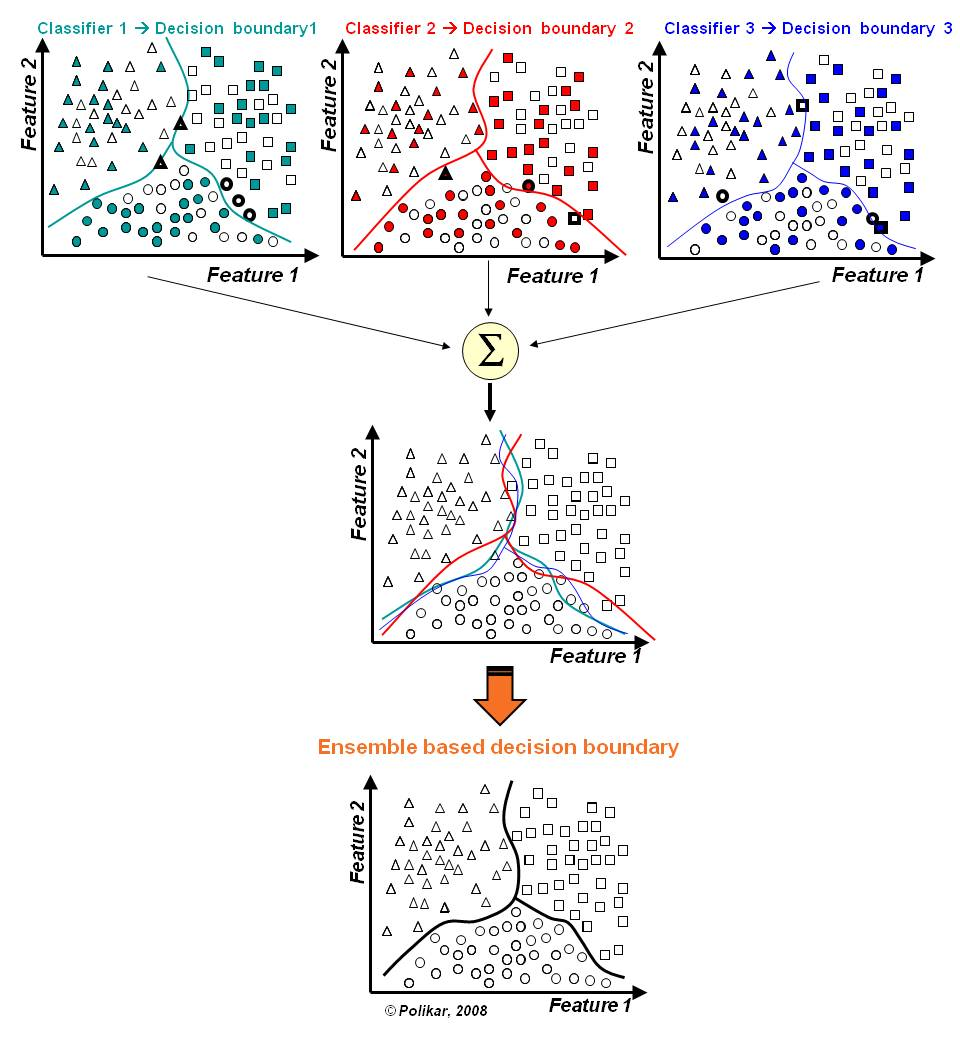
\includegraphics[scale=0.35]{Combining_classifiers2}
\caption{The combination of classifiers with different decision boundaries improves predictive power \citep{polikarphoto}.}
\label{fig:diversity}
\end{figure}

Bagging, \textbf{B}ootstrap \textbf{agg}regat\textbf{ing}, originally refers to the training of classifiers of one type on random resamples of the training data \citep{Breiman1996}. For the training of $k$ classifiers, $k$ training sets of size $N$ are generated by drawing from the original data set of size $N$ with replacement. While the individual classifiers' errors on the test set increase with that technique due to overfitting to the samples that occur more often in the training set, the combination of these overfitted classifiers makes the ensemble so strong \cite{krogh1996learning}.

An alternative to Bagging is Boosting where in a sequence of classifiers, incorrectly classified samples are resampled more often to improve the accuracy of the single classifier \cite[p. 173]{opitz1999popular}. Since 1996 both Bagging and Boosting have been expanded and applied at different steps of the classifier learning and final ES. Opitz and Maclin show that combining different classifiers that are trained on the same data, too, produces very good results \cite[p. 170]{opitz1999popular}. \\

One potential issue in ES is overfitting, i.e. the inclusion of many classifiers in the ensemble may produce good results on the training set but result in poor performance on the test set \cite[p. 253]{sun2011bagging}, \cite[p. 2092]{cawley2010over}. To prevent this, \cite{caruana2004ensemble} present a novel approach. They extend the simple iterative inclusion or exclusion of classifiers to an ensemble in three ways: 
\begin{description}
	\item[Selection with Replacement] Classifiers can be included in the ensemble several times meaning that good classifiers can be picked again instead of poorer ones when the initial top $t$ models have already been selected.
	\item[Sorted Ensemble Initialization] Instead of filling an empty ensemble, the initial ensemble is already comprised of the $t$ best classifiers and filled from there on.	
	\item[Bagged ES] In this case, instead of bagging the training data, subsets of classifiers are created. One then optimizes the classifier combination within the subset and results across all subsets are averaged to obtain the final ensemble.
\end{description}
As a demonstration of bagged ES, imagine that one draws 15 samples from a classifier library of 1000 with a probability $p =0.5$ such that each sample or bag contains 500 classifiers whose combination is then optimized with, for example, forward-selection. The 15 obtained sub-ensembles are then combined \cite[p. 3]{caruana2004ensemble}.
The empirical results of Caruana et al. point strongly towards setting the ratio of models per bag to 0.5 as it shows the strongest advantage over the baseline best model. They also show that ensemble selection works extremely well with any type of performance metric, \mbox{i.e. }accuracy, ROC, root mean-squared error, \mbox{etc. }and accounted for one third of the total 8.7\% outperformance of ES over the best model alone. Caruana et al. optimized the ES with forward stepwise selection where one iteratively adds classifiers until the performance converges. However, any selection or optimization procedure is possible. Linear methods include taking the simple average, the weighted average, or the median. Voting covers majority voting, plurality voting for multi-class problems, or weighted voting. For a more detailed view on ensemble combination see Chapter 4 in \cite{zhou2012ensemble}. Usually, the classifiers are combined with regards to some objective function, the ensemble accuracy for example. 

The problem of optimizing the classifier combination with regards to some objective function is a non-linear problem. A possible search heuristic for finding the optimal classifier combination are Evolutionary Algorithms, a class of algorithms that emulate different behavior found in nature: the evolution of genes or individuals over time or the movement of swarms or flocks. EAs solve the initial questions of which models to include and how to combine them heuristically and have shown competitive results in the past \citep{oliveira2005multi}.


%Probably add here: 'Overfitting cautious selection of classifier ensembles with genetic algorithms' by Santos:
%' However, even though the control of overfitting is a challenge in machine learning problems, much less work has been devoted to the control of overfitting in selection tasks. The objectives of this paper are: (1) to show that overfitting can be detected at the selection stage; and (2) to present strategies to control overfitting. Decision trees and k nearest neighbors classifiers are used to create homogeneous ensembles, while single- and multi-objective genetic algorithms are employed as search algorithms at the selection stage. In this study, we use bagging and random subspace methods for ensemble generation. The classification error rate and a set of diversity measures are applied as search criteria. We show experimentally that the selection of classifier ensembles conducted by genetic algorithms is prone to overfitting, especially in the multi-objective case. In this study, the partial validation, backwarding and global validation strategies are tailored for classifier ensemble selection problem and compared.'



\section{Using Evolutionary Algorithms for Ensemble Selection}
\label{UsingEA}
Ensemble Selection is essentially an optimization problem in a constrained search space. In order to find an effective solution, optimization strategies must exploit all available information. One can use derivative-based information, i.e. on the gradient of the search space. In the case of complex spaces with many local optima, these methods tend to get stuck and miss global solutions. Evolutionary Algorithms capitalize on a different strategy that often makes a suitable trade-off between exploration and exploitation of the search space. Hence, they are a search heuristic worthwhile exploring for ensemble selection.

\subsection{Introduction to Evolutionary Algorithms}
\label{introEA}
Evolutionary Algorithms are nature-inspired optimization algorithms. The idea of emulating natural selection and evolution emerged very early into the development of computational optimization; already in the 1950s, first evolution systems were employed to optimize real-valued functions \cite[p. 2]{mitchell1999introduction}. The first genetic algorithm that mimics the way genes on a chromosome are encoded, was developed by John Holland in the 1960s. In his book \emph{Adaptation in natural and artificial systems}, Holland presented an advanced, more abstract version of the GA that is able to solve many different problem along with a theoretical framework of how GAs optimize \citep{holland1975adaptation}. Genetic Algorithms still follow the structure presented by \citeauthor{holland1975adaptation}. As many terms are derived from biology and might deserve explanation, some concepts and vocabulary are briefly here. EAs are \emph{population}-based, where the population is a group of candidate solutions to the problem at hand. The population can also be called swarm and its size is denoted by $N$. The candidate solution is usually called \emph{chromosome}, but also particle, individual or string. It can be a binary-encoded or a real-valued numeric vector. The candidate solution consists of positions of \emph{genes}, \emph{loci} and contains as many loci as the problem has dimensions. The value at each locus is called \emph{allele}. As an example, in the case of ensemble selection, the problem dimension is equal to the number of models $D$ in the model library. So each chromosome $x$ consists of $D$ genes and the value at $x_i$ corresponds to the weight assigned to model $i \in 1,\dots, D$.

Typically, EAs consist of five stages which are explained here with the example of the canonical Genetic Algorithm: 1. Initialization, where the initial population of dimensions $N \times D$ is randomly created. 2. Evaluation: its fitness is evaluated on some cost function to be optimized. 3. Selection: a fixed number of best performing chromosomes is selected for the next stages. 4. Crossover: two chromosomes are randomly selected and combined to produce offspring. 5. Mutation: the offspring is randomly mutated and included in the population. The steps 2--5 are repeated until a stopping criterion is reached, e.g. the optimum, a fixed number of generations or a convergence criterion.

This basic setup can be varied and extended in numerous ways. Instead of random selection, one can implement fitness-proportionate selection or roulette-wheel selection, where better performing solutions are assigned a higher probability of selection. An alternative is tournament selection where randomly chosen chromosomes "perform again" each other and the best individuals are selected \citep{miller1995genetic}.
There are many options on how to combine the parents to produce offspring, the simplest one being one-point crossover where both parents are split at a random point $i \in 1,\dots, D$ and the first child inherits the characteristics of the first parent up until $i$ from where on it posses the second parent's properties. The inverse is applied to the second child. Another common modification is elitism where a fixed number of best evaluated chromosomes in each generation are preserved and replace the worst performing chromosomes in step 5 and are directly transferred to the next generation. \\



%Considering 
%invalid solutions
%canonical
%implicit parallelism
% too much exploitation: local hillclimbing; too much exploration: loss of valuable information
% cite De Jong 1993 about  p. 14 % which is better
%Additionally, evolutionary algorithms can either optimize binary encoded solutions as well as real-valued solutions. This is representative of the major advantage of evolutionary algorithms compared to other optimization strategies: its adaptiveness. Most evolutionary algorithms fail to find the global optimum (citation), but they are well versed to solve a range of problems and find sufficiently satisfying solutions.

%"A genetic algorithm maintains a population of potential solutions to the objective function being optimized. The initial group of potential solutions is determined randomly. These potential solutions, called "chromosomes," are allowed to evolve over a number of generations. At every generation, the fitness of each chromosome is calculated. The fitness is a measure of how well the potential solution optimizes the objective function. The subsequent generation is created through a process of selection and recombination. The chromosomes are probabilistically chosen for recombination based upon their fitness; this is a measure of how well the chromosomes achieve the desired goal (e.g. find the minimum in a specified function, etc.). The recombination operator combines the information contained within pairs of selected "parents", and places a mixture of the information from both parents into a member of the subsequent generation. Selection and recombination are the mechanisms through which the population "evolves." Although the chromosomes with high fitness values will have a higher probability of being selected for recombination than those which do not, they are not guaranteed to appear in the next generation. The "children" chromosomes produced by the genetic recombination are not necessarily better than their "parent" chromosomes. Nevertheless, because of the selective pressure applied through a number of generations, the overall trend is towards better chromosomes.
%In order to perform extensive search, genetic diversity must be maintained. When diversity is lost, it is possible for the GA to settle into a sub-optimal state. There are two fundamental mechanisms which the basic GA uses to maintain diversity. The first, mentioned above, is a probabilistic scheme for selecting which chromosomes to recombine. This ensures that information other than that represented in the best chromosomes appears in the subsequent generation. Recombining only good chromosomes will very quickly converge the population without extensive exploration, thereby increasing the possibility of finding only a local optimum. The second mechanism is mutation; mutations are used to help preserve diversity and to escape from local optima. Mutations introduce random changes into the population.
EAs are often used in the following scenarios: the problem is very complex or high-dimensional. Also, because they work heuristically and not analytically, discontinuous or non-differentiable objective functions are not an issue to their performance as opposed to derivative-based algorithms. Also, as EAs can deal with the exploration/exploitation trade-off quite well so that search spaces with many local optima do not necessarily impede their convergence. 
Nevertheless, one needs to bear in mind that EAs do not find the analytical function optimum. With finite populations, they may never reach the global optimum or lose it over time due to mutation. EAs are best applied in situations where a reasonably satisfying solution in a reasonable time frame is sufficient. As De Jong argues: the genetic algorithm "is attempting to maximize cumulative payoff from arbitrary landscapes, deceptive or otherwise. In general, this is achieved by not investing too much effort in finding cleverly hidden peaks (the risk/reward ratio is too high)." \cite[p. 15]{de1993genetic}. This notion can be transferred to all EAs \cite[p. 92]{mitchell1999introduction}.\\ %some of the pioneering work [Holland, 1975]
%In order to control this, their parameters must be carefully tuned. A large enough population size for example can help maintain many diverse solution. \\


%Considering the somewhat random nature of how EAs find and maintain solutions, the question rises of why one would expect EAs to outperform any other heuristic algorithm at all. Even more so, as EAs make no assumption on the search space and exploit only the information contained the obtained fitness values to guide their search. HowevAny effective search is based on the tension between exploration and exploitation. Exploration refers to the moving around in the search space to find new information and potentially find global peaks. Exploitation is the use and propagation of local information \cite[p. 64]{karr1999practical}. 

%Why would we ever expect a GA to outperform RMHC on a landscape like R1? In principle, because of implicit parallelism and crossover. If implicit parallelism works correctly on R1, then each of the schemas competing in the relevant partitions in R1 should have a reasonable probability of receiving some samples at each generation—in particular, the schemas with eight adjacent ones in the defining bits should have a reasonable probability of receiving some samples. This amounts to saying that the sampling in each schema region in R1 has to be reasonably independent of the sampling in other, nonoverlapping schema regions. In our GA this was being prevented by hitchhiking—in the run represented in figure 4.2, the samples in the s3 region were not independent of those in the s2 and s4 regions. In RMHC the successive strings examined produce far from independent samples in each schema region: each string differs from the previous string in only one bit. However, it is the constant, systematic exploration, bit by bit, never losing what has been found, that gives RMHC the edge over our GA. %Mitchell 99




%principies of natural selection and genetic recombination.

%The GAs described in the current literature are highly modified to reconcile the differences between function optimization, in which the effectiveness is measured by the best solution found, and maximizing cumulative returns, in which finding the absolute best solution may not be the only critical issue. %Baluja p.5










\subsection{Optimizing Ensemble Selection}
\label{subop}
When using EAs, two fundamental questions need to be decided upon at the start: the function to be optimized and the encoding. EAs can be binary-encoded, meaning that each gene on the chromosome is either 0 or 1. In the case of Ensemble Selection, a 0 at $x_i$ means that the model $i \in 1,\dots D$ is not included and vice versa. For the evaluation the 1's are divided by their sum, i.e. an exemplary vector $x = {01101}$ of dimensions $(1\times 5)$ is divided by the number of 1's, 3 in this case, such that the weights sum up to 1. As an alternative, the solution vector can be real-valued or numerical. Instead of 0/1, the value at $x_i$ can be any value within the boundary, which in the case of ES is confined to $[0,1]$. As the weights need to sum up to 1, they are divided by their cumulative sum. As an example, a preliminary solution vector $x = \{0.1, 0.5, 0.8, 0.2, 0.05\}$ is divided by its sum 1.65 so that the final solution vector is $x = \{0.06, 0.3, 0.48, 0.12, 0.03\}$. To prevent the EAs from including a large number of arbitrarily small weights, sparsity rules can be enforced where weights smaller than 1\% can be excluded. 
%In order to find the optimal weights for the ensemble selection problem, a number of different evolutionary algorithms was considered, each with particular properties that might prove helpful in solving the optimization problem at hand. In the sections below, each of them are shortly introduced. 
Depending on the problem and the encoding, one potential issue with EAs is the production of invalid solutions, as especially the mutation step can change solutions such that they are outside of the defined constraints. In the case of ensemble weights, these constraints are $0 \leq w_i \leq 1$ and $\sum_{i = 1}^{D} w_i = 1$. 

EAs in general have a tendency to overfit and there is some experimental evidence that they overfit ensemble selection problems (\cite{Robilliard2002}, \cite{radtke2006impact}, \cite{dos2009overfitting}). Complex validation strategies can be implemented to prevent this; their performance however is not overly effective and the effect size of overfitting is rather small \cite[p. 1424]{dos2008overfitting}. In this paper, bagging as described by \cite{caruana2004ensemble} is implemented to test whether a) overfitting is an issue and b) if it can be mitigated by bagging and c) whether bagging improves the solutions.


\newpage
\section{Algorithms implemented}
\label{alg}
While various EA are suitable for optimizing ES, the final selection for this study consists of the Genetic Algorithm (GA), the Backtracking Search Algorithm (BSA), Population-based Incremental Learning (PBIL) and Particle Swarm Optimization (PSO). As a benchmark of performance Hil-Climbing and Stochastic Hill-Climbing are implemented.

\subsection{Genetic Algorithm}
%\ref{GA}
As the Genetic Algorithm (GA) has already been explained in its canonical form in Section \ref{introEA} as a prototype of EAs, it will not be dealt with in much detail. For the ES case, a GA with elitism, one-point crossover and roulette-wheel selection is implemented.


\subsection{Backtracking Search Optimization Algorithm}
%ref{BSA}
The Backtracking Search Optimization Algorithm (BSA) is comparatively new algorithm that was introduced in 2013 to solve numerical problems \citep{civicioglu2013backtracking}. Out of all the algorithms taken into account, it can be considered the``sleekest" with only one control parameter. Additionally to the GA phases, a second Selection stage is implemented at the very beginning where an old population is maintained such that the BSA population preserves a memory. 
After initialization follows the new selection stage where the historical population is randomly updated according to $\textit{if } a < b  \:|\: a,b \sim U(0,1 )$. It is then permuted and Mutation and Crossover follow. The population is mutated based on Equation (\ref{eqbsa1}):
\begin{equation} \label{eqbsa1}
\textit{Mutant} = \textit{Population} + F \cdot (\textit{historical Population} - \textit{Population})
\end{equation}
where $F = 3 \cdot \varepsilon$, $\varepsilon \sim N(0,1)$.
The original BSA is developed for numerical, real-valued problems but it can easily be adapted to binary encoding.

\subsection{Population-Based Incremental Learning}
%ref{PBIL}
The Population-Based Incremental Learning Algorithm (PBIL) by \cite{baluja1994population} can be considered an abstraction of the GA as it drops the population. Instead, it uses a probability vector from which population samples are drawn. This vector denotes the probability of a certain value appearing at a certain position of the solution vector. In a binary setting of the PBIL, the probability vector of a population denotes the probability of a 1 appearing at position $i$ of the candidate solution $x$. Instead of recombination to obtain solutions with high fitness, the probability vector from which the population is drawn is gradually shifted towards solutions with high fitness \cite[p. 11]{baluja1994population}. The vector is initialized with 0.5 and is updated by the following rule:
\begin{equation}
p_i = p_i \cdot (1 - \gamma) + (\gamma \cdot x_i),
\end{equation}
where $p_i$ is the probability of generating a 1 bit at position $i$, $x_i$ is the solution vector at position $i$ towards which the probability vector at $i$ is moved and $\gamma$ is the learning rate. The learning rate affects how quickly the probability vector moves towards a feasible solution, i.e. how informative the previous search is. As such, it controls the trade-off between exploration and exploitation and premature convergence. It is usually suggested to set the learning rate to values around 0.1, as higher values lead to an early search focus whereas lower values enable greater search exploration, which is preferable when there is no certainty on the prevalence of local optima. \cite[p. 16--17]{baluja1994population}.
It should be noted that the PBIL and the probability vector so far are as described in \cite{baluja1994population}, meaning that only binary encoding is considered. The PBIL, however, can be adapted to real-valued encoding, thus making the implication of a probability vector more complicated. 

As a solution, \cite{servet1997telephone} suggest an interval-based probability vector. It is assumed that the solution is continuous and bounded, such that for each position $i$, an bounded interval $[low_i, up_i]$ can be defined. The value at position $i$ of the probability vector then denotes the probability that $x_i$ is greater than a threshold. The initial threshold is defined as $\frac{low_i + up_i}{2}$ and is updated throughout the iterations. If $p_i \geq 0.9$, i.e. the probability that $x_i$ is greater than the threshold is $\geq 0.9$, the threshold is updated to $\frac{\frac{low_i + up_i}{2} + up_i}{2}$, i.e. $low_i$ is updated to the previous threshold and $p_i$ is reinitialized at 0.5. Both $p_i$ and the $up_i$ are updated equivalently whenever $p_i \leq 0.1$. In the case of ES in this pape, the interval is slightly redefined from $\frac{low_i + up_i}{2}$ to $\frac{low_i + up_i}{\sum{i}}$ such that the initial probability assumes equal weights.



\subsection{Particle Swarm Optimization}
%ref{PSO}
The Particle Swarm Optimization Algorithm (PSO) draws on swarm intelligence to find the optimum. The candidate solutions, called particles, move through the search space by random mutations, called velocities. The velocity of each particle consists of three components: an inertia weight, i.e. the "unwillingness" of a particle to leave its current position which also prevents it from moving too erratically, a cognitive component, i.e. the particle's ability to remember a previous good solution, and a social component, i.e. the particle's ability to move towards optimal solutions found by its neighbors in the swarm. 
The PSO was introduced in 1995 by Kennedy and Eberhart and simulates the social behavior of bird flocking or fish swarming. 
The particles evolve by the following equations:
\begin{align}
v_{i,t+1} &= \gamma v_{i,t} + \varphi_1 \delta(0,1)(P_i - x_{i,t}) + \varphi_2 \delta(P_g - x_{i,t})\\
x_{i,t+1} &= x_{i,t} + v_{i,t+1}
\end{align}
where $\delta \sim U(0,1)$, $x_{i,t}$ is the value at position $i$ and time step $t$ of the candidate solution $x$, $P_i$ refers to the previously best personal solution and $P_g$ denotes the best solution in the neighborhood. \\
The inertia weight $\gamma$ controls how fast each particle moves and was not in the proposition for the original PSO \citep{kennedy1995}. It was added three years later as it adds significantly to the algorithm's ability to search and exploit the search space \cite[p. 70]{shi1998modified}. For $\gamma > 1.2$ the swarm keeps on exploiting new search areas, for $\gamma < 0.8$ it exploits local areas more and finds the balance between the two for values $0.8 < \gamma < 1.2$ However, experimental studies have shown that non-fixed $\gamma$ values also perform extremely well and that the so called random inertia weight $\gamma = 0.5 + \delta/2$ performs well on a number of different problems \cite[p. 643]{bansal2011inertia}.
$\varphi_1$ and $\varphi_2$, the acceleration coefficients control the influence of information on the movement of the particles. Usually, one sets $\varphi_1 = \varphi_2$ to values around 2 \cite[p. 1946]{kennedy1995}. \\
Additionally, the information neighborhood of each particle, also called topology, is not a trivial setup as it determines how much information is available to each particle. The two most common ones are the \textit{lbest} and \textit{gbest} topologies but there are many other variants. In the \textit{lbest}, each particle $i$ is informed on its own position and its two adjacent neighbors, resulting in a ring lattice (see Figure \ref{Fig:topo}). In a \textit{gbest} setting, which is also the setting in the initial algorithm, the particles are informed by the global neighborhood. The information flow in this social network influences the convergence behavior strongly: In a study by \cite{kennedymendes}, different topologies were evaluated and \textit{gbest} performed worst in both accuracy and speed, while \textit{lbest} performed slightly better when removing particle $i$ (the self) from the information \cite[p. 1674]{kennedymendes}. For this paper, both the \textit{gbest} and \textit{lbest} without self are tested; more complex topologies von Neumann neighborhood were not considered due to the popularity of the former and the complexity of the latter.

\begin{figure}[ht]
	\begin{center}
		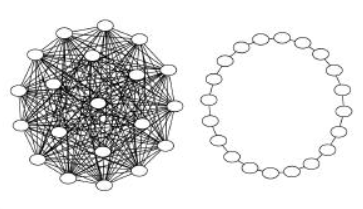
\includegraphics[scale=0.9]{topology}
		\caption{A visualization of the \textit{gbest} and \textit{lbest} topologies \cite[p. 1671]{kennedymendes}.}
		\label{Fig:topo}
	\end{center}
\end{figure}



\subsection{(Stochastic) Hill-climbing}
Simple Hill-climbing is an iterative search algorithm that does not belong to the class of evolutionary algorithms. It is, however, a powerful and fast algorithm that XXX.
HC systematically modifies an initial candidate solution in directions that yield higher fitness values. If the first modification did not improve the current fitness value, the solution moves into another direction. Ideally, in a convex space with only one optimum, HC returns the hill-top, the best solution after a fixed number of iterations \cite[p. 252]{skiena2008algorithm}. As solutions with lower fitness values are not further investigated, HC is prone to get stuck in local optima as it cannot return to previous points and must go upwards \cite[p. 113]{russell1995modern}. 
One resolution to mitigate this problem is Stochastic Hill-climbing where a random neighbor around the current solution is selected and evaluated. If it yields higher fitness, it replaces the current solution. instead of systematic mutation, randomly mutated candidate are evaluated and accepted if they yield a higher fitness. With this probabilistic element, the HC is forced to consider solutions further away from the current solution.

Both the simple HC and the SHC are simple to implement and perform very well on a number of optimization problems \citep{Jacobson2004}. They are often used as benchmark comparisons because one can justify (or fail to justify) the use of more complex algorithms like EAs when simpler and faster methods like HC perform competitively (\cite{mitchell1993will}, \cite{wattenberg1996stochastic}, \cite{PRUGELBENNETT2004135}).





\section{Experimental Design}
\label{design}
All algorithms were hand-coded in R and tested on the publicly available data from the DATA MINING CUP 2016 on fashion retail returns was used \citep{dmcdata}. As in the contest submissions of Humboldt University of Berlin, a model library of 26 Random Forests and 26 XGBoost, 54 models in total, was used. 
The high server usage at the Research Data Center at Humboldt University where all computations for this paper were handled limited both the variety of different parameter settings, the number of iterations and the data sets on which the algorithms were run. 
To deal with these restrictions, the DMC data set was reduced to 30\% of its original size. This sub-set was then split into a training and a validation set with a 70/30 ratio, so that each algorithm optimized on 372,000 predictions. The evaluation of the optimization function, which is usually called several times in each iteration of the evolutionary algorithms is quite computationally expensive, so that even with the reduced data set, the number of iterations was limited to 500.


Each configuration of the five evolutionary algorithms was optimized in four seperate experiments: 1. binary-encoded, 2. real-valued, 3. binary-encoded + Bagging and 4. real-valued + Bagging. Bagging used of ten bags each.

All experiments followed the same structure: the solution populations were optimized over 500 generations (or iterations) where their performance was evaluated on a validation set. As a performance measure, the Brier Score was used, which can be intuitively understood a version of the Mean Squared Error for binary outcomes. It is defined as:
\begin{equation}
BS = \frac{1}{N} \sum_{i = 1}^{N} (p_i - o_i)^2
\end{equation}
where $N$ denotes the sample size, $p_i$ is the predicted probability and $o_i$ is the actual binary outcome (i.e. 1 or 0). The Brier Score lies in the [0,1] interval where a low value indicates a good forecast and the higher the Brier Score, the poorer the forecast performance. In the Bagging experiments, each algorithm is optimized on ten different subsets of the full classifier set and the results are then averaged.
Additionally, the ensemble weights yielded by the algorithms were tested on the classification set of the DMC. The results for this data were recently published and are available on the DMC website.
\begin{table}[ht]
	\centering
	\begin{tabular}{llcccc}
		\hline
		
		Algorithms& Abbr. & Psize & \multicolumn{3}{c}{Parameters} \\ 
		\hline
		& & & Mixrate& & \\
		\multirow{2}{*}{BSA} & BSA1 & 30 & 1 && \\ 
		& BSA2 & 100 & 1&& \\ \hline
		& & & Crossover & Elitism & pMutation \\
		\multirow{4}{*}{GA}  & GA1 & 30 & 0.50 & 0.03 & 0.05 \\ 
		& GA2 & 100 & 0.50 & 0.03 & 0.05 \\ 
		& GA3 & 30 & 0.80& 0.03 & 0.05 \\ 
		& GA4 & 100 & 0.80& 0.03 & 0.05 \\ \hline 
		 &&& Learning Rate & Shift & Prob \\
		\multirow{4}{*}{PBIL} & PBIL1 & 30 & 0.05& 0.05 & 0.02 \\ 
		& PBIL2 & 100 & 0.05 & 0.05 & 0.02\\ 
		& PBIL3 & 30 & 0.10& 0.05 & 0.02 \\ 
		& PBIL4 & 100 & 0.10 & 0.05 & 0.02 \\ \hline 
		 &&& Phi & Inertia & Initial Speed \\
		\multirow{4}{*}{PSO-G} & PSOG1 & 30 & 1.80 & 0.5 + $\delta$/2 & 0.01 \\ 
		&PSOG2 & 100 & 1.80& 0.5 + $\delta$/2 & 0.01 \\ 
		&PSOG3 & 30 & 2.10 & 0.5 + $\delta$/2 & 0.01\\ 
		&PSOG4 & 100 & 2.10& 0.5 + $\delta$/2 & 0.01 \\ \hline
		 &&& Phi & Inertia & Initial Speed \\
		\multirow{4}{*}{PSO-L} & PSOL1 & 30 & 1.80& 0.5 + $\delta$/2 & 0.01 \\ 
		& PSOL2 & 100 & 1.80& 0.5 + $\delta$/2 & 0.01 \\ 
		& PSOL3 & 30 & 2.10 & 0.5 + $\delta$/2 & 0.01\\ 
		& PSOL4 & 100 & 2.10 & 0.5 + $\delta$/2 & 0.01 \\ 
		\hline
	\end{tabular}
\caption{The parameter configurations for each variant of the five evolutionary algorithms run; $\delta \sim U(0,1)$}
\label{tbl:params}
\end{table}



\newpage
\section{Results}
\label{results}
The runtime of the algorithms was an unpleasant surprise and is most likely due to the high server usage at the RDC as test runs with a small number of iterations finished quickly on standard laptops. In the final run, each configuration took approximately 23 hours to run, whereas the bagged implementations took 27 hours on average. The binary-encoded variants ran a bit faster as their code was slightly less complex than their real-valued counterparts but still took 21 hours.

Figures \ref{fig:exp12} and \ref{fig:exp34} show the average convergence of each algorithm across all parameter settings. The GA and BSA converge as expected, whereas both PSO implementations show only little improvement to their random initialization. The PBIL is seemingly unable to hold any good solutions over time and tried solutions in a random walk fashion. The parameter setting might be at fault here as the bagged experiments yielded very similar results. %WHERE DID I GET THE PARAMS FROM?

%PSOG SO POORLY
%BAGGING WORSENED HC

\begin{figure}
\centering %CHANGE SUBCAPTION
	\begin{subfigure}{.5\textwidth}
		\centering
		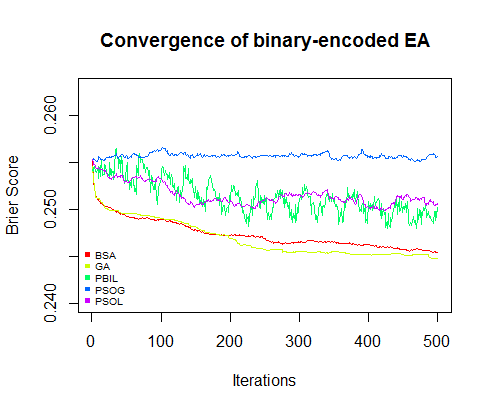
\includegraphics[width=\linewidth]{Conv_N_bin_EA}
		%\caption{A subfigure}
		\label{fig:nb}
	\end{subfigure}%
	\begin{subfigure}{.5\textwidth}
		\centering
		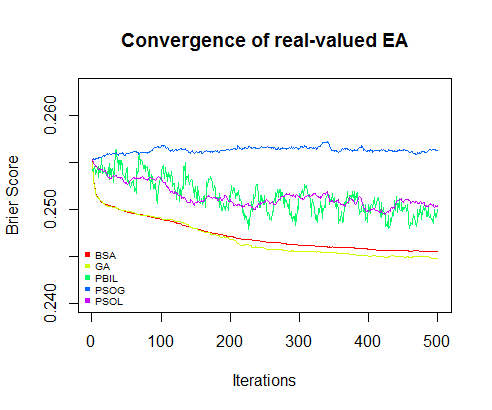
\includegraphics[width=\linewidth]{Conv_N_real_EA}
		%\caption{A subfigure}
		\label{fig:nr}
	\end{subfigure}
	\caption{Convergence Results of Experiments 1 and 2.}
	\label{fig:exp12}
\end{figure}

\begin{figure}
	\centering
	\begin{subfigure}{.5\textwidth}
		\centering
		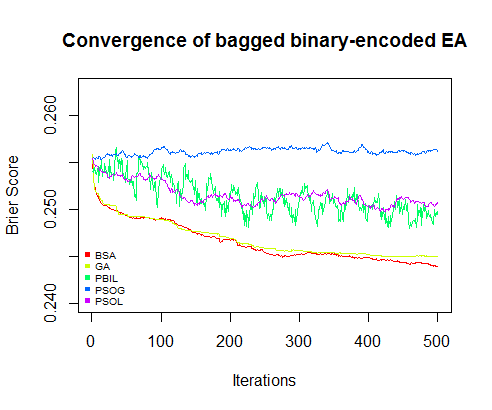
\includegraphics[width=\linewidth]{Conv_bin_bag}
		%\caption{A subfigure}
		\label{fig:bb}
	\end{subfigure}%
	\begin{subfigure}{.5\textwidth}
		\centering
		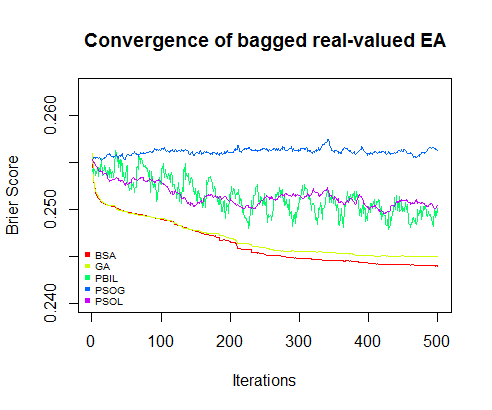
\includegraphics[width=\linewidth]{Conv_real_bag_EA}
		%\caption{A subfigure}
		\label{fig:br}
	\end{subfigure}
	\caption{Convergence Results of Experiments 1 and 2.}
	\label{fig:exp34}
\end{figure}

\begin{table}[ht]
	\centering
	\begin{tabular}{lccllcc}
		\hline
		Algorithms & ES (binary) & ES (real) & $\mid$ & Algorithms & ES (binary) & ES (real) \\ 
		\hline
		BSA1 & 5 & 26 && PSOG1 & 8 & 13 \\ 
		BSA2 & 3 & 13 & &PSOG2 & 6 & 14 \\ 
		BSA.BAG1 & 9 & 18 && PSOG3 & 5 & 7 \\ 
		BSA.BAG2 & 3 & 6 & &PSOG4 & 2 & 4 \\ 
		GA1 & 4 & 4 & &PSOG.BAG1 & 7 & 10 \\ 
		GA2 & 5 & 5 & &PSOG.BAG2 & 3 & 5 \\ 
		GA3 & 4 & 5 & &PSOG.BAG3 & 4 & 4 \\ 
		GA4 & 3 & 3 & &PSOG.BAG4 & 2 & 4 \\ 
		GA.BAG1 & 2 & 3 && PSOL1 & 4 & 5 \\ 
		GA.BAG2 & 3 & 4 && PSOL2 & 6 & 8 \\ 
		GA.BAG3 & 2 & 3 & &PSOL3 & 3 & 12 \\ 
		GA.BAG4 & 3 & 4 & &PSOL4 & 7 & 8 \\ 
		PBIL1 & 9 & 17 & &PSOL.BAG1 & 4 & 6 \\ 
		PBIL2 & 3 & 26 & &PSOL.BAG2 & 6 & 6 \\ 
		PBIL3 & 7 & 9 & &PSOL.BAG3& 2 & 7 \\ 
		PBIL4 & 7 & 9 && PSOL.BAG4 & 5 & 11 \\ 
		PBIL.BAG1 & 8 & 12 && SHC & 3 & \\ 
		PBIL.BAG2 & 5 & 16 && SHC.BAG & 11 & \\ 
		PBIL.BAG3 & 6 & 7 && HC & 2 & \\ 
		PBIL.BAG4 & 7 & 8 && HC.BAG & 6 & \\ 
		\hline
	\end{tabular}
	\caption{Ensemble Sizes Chosen by the EA}
	\label{tbl:es}
\end{table}

The algorithms yield strongly varying results in terms of ensemble sizes. Some variants pick as many as 26 of the 54 classifiers, whereas others decide on only 2 - 3. A complete overview can be found in Table \ref{tbl:es}. Some results by \cite{opitz1999popular} indicate that the marginal benefit of inclusion is highest for the first few models in the ensemble and decreases quickly \cite[p. 190]{opitz1999popular}. Even though the classifiers in the library can be considered diverse due to their wide parameter range, it is intuitive that after a certain number of RF and XGBoost models in the ensemble, the performance does not improve anymore and the errors increase. The correlation of performance and ensemble size which is evident from Figure \ref{fig:perfsize} is extremely interesting: For both the binary- and the real-coded versions, sparse solutions tend to yield better results. Still, the error rate increases quicker in the binary case. This should not come as a surprise because real-valued solutions may include many classifiers, many of them by a small weight only, so they do not decrease the performance. In the binary case, the weights are less likely to be arbitrarily small so any classifier in the ensemble has a larger relative weight. 

\begin{figure}[ht]
	\begin{center}
		\includegraphics[scale=0.8]{Perform_size}
		\caption{A scatterplot of the error rate on the ensemble size.}
		\label{fig:perfsize}
	\end{center}
\end{figure}

The complete results of the experiments can be found in Table \ref{tbl:perf}, where the columns refer to the performance on the validation and classification set. The best performing configurations for each of the two data sets are printed in boldface. When two scores were equal, both are emphasized. Overall, the real-valued solutions tend to perform slightly better than their binary counterparts. 
 
In training, the bagged GA yields the best results with BSA and the PSO-L being very comparatively in their error rate. Interestingly, the population size has opposing effects on the performance across algorithms. Overall, the GA performs better with a small population size whereas the increase of solution vectors in the population yields a performance increase for all others. As was somewhat expected after reading the paper by \cite{kennedymendes}, the PSO-G with a global information topology performs the worst out of all the configurations.

When compared to the baseline evaluations, the EAs do not measure up. All solutions, even the best solutions have a notable increase in the BS compared to the single best model. Even a simple average of the four best models outperforms 31 of the binary and 28 of the real-valued solutions. Interestingly, both HC and SHC suffer from bagging and yield best results on the full model library. HC maintains the error rate of the best performing model by only adding another classifier to the ensemble, with SHC also only considering three classifiers. Both the HC and SHC weigh the two classifiers more cleverly than the bagged GA1 and GA3 which also only include two classifiers.%PERCENTAG EWRONG

This paper also considered the problem of overfitting, so that the results of applying the ensemble weights to the classification data are surprising. Five binary and four real-valued solutions yield BS that are significantly lower than the single best classifier. HC and SHC only perform as good as the best model and do not lower the BS further.  

\begin{table}[ht]
	\centering
	\begin{tabular}{lcccc}
		\hline
		& \multicolumn{2}{c}{BS on Validation} & \multicolumn{2}{c}{BS on Classification} \\
		\cline{2-5}
		Algorithms & Binary & Real & Binary & Real \\ 
		\hline
		BSA1 & 0.2413 & 0.2466 & 0.2951 & 0.3007 \\ 
		BSA2 & 0.2396 & 0.2419 & \textbf{0.2945} & 0.2957 \\ 
		BSA.BAG1 & 0.2454 & 0.2446 & 0.2986 & 0.2980 \\ 
		BSA.BAG2 & 0.2396 & 0.2403 & \textbf{0.2945} & 0.2953 \\ 
		GA1 & 0.2416 & 0.2395 & 0.2954 & 0.2947 \\ 
		GA2 & 0.2413 & 0.2407 & 0.2951 & 0.2949 \\ 
		GA3 & 0.2406 & 0.2402 & 0.2948 & 0.2947 \\ 
		GA4 & 0.2430 & 0.2402 & 0.2966 & 0.2951 \\ 
		GA.BAG1 & \textbf{0.2393} & \textbf{0.2391} & 0.2946 & 0.2947 \\ 
		GA.BAG2 & 0.2445 & 0.2402 & 0.3008 & 0.2961 \\ 
		GA.BAG3 & \textbf{0.2393} & \textbf{0.2391} & 0.2946 & \textbf{0.2946} \\ 
		GA.BAG4 & 0.2445 & 0.2418 & 0.3008 & 0.2980 \\ 
		PBIL1 & 0.2516 & 0.2516 & 0.3051 & 0.3049 \\ 
		PBIL2 & 0.2396 & 0.2466 & \textbf{0.2945} & 0.3007 \\ 
		PBIL3 & 0.2469 & 0.2452 & 0.3017 & 0.3001 \\ 
		PBIL4 & 0.2467 & 0.2426 & 0.3000 & 0.2972 \\ 
		PBIL.BAG1 & 0.2513 & 0.2512 & 0.3054 & 0.3048 \\ 
		PBIL.BAG2 & 0.2458 & 0.2454 & 0.3003 & 0.2995 \\ 
		PBIL.BAG3 & 0.2485 & 0.2436 & 0.3029 & 0.2988 \\ 
		PBIL.BAG4 & 0.2467 & 0.2428 & 0.3000 & 0.2974 \\ 
		PSOG1 & 0.2489 & 0.2475 & 0.3051 & 0.3035 \\ 
		PSOG2 & 0.2482 & 0.2477 & 0.3047 & 0.3037 \\ 
		PSOG3 & 0.2460 & 0.2527 & 0.3022 & 0.3097 \\ 
		PSOG4 & 0.2619 & 0.2617 & 0.3195 & 0.3192 \\ 
		PSOG.BAG1 & 0.2506 & 0.2479 & 0.3071 & 0.3040 \\ 
		PSOG.BAG2 & 0.2486 & 0.2526 & 0.3028 & 0.3070 \\ 
		PSOG.BAG3 & 0.2479 & 0.2541 & 0.3047 & 0.3115 \\ 
		PSOG.BAG4 & 0.2619 & 0.2617 & 0.3195 & 0.3192 \\ 
		PSOL1 & 0.2452 & 0.2405 & 0.2978 & 0.2957 \\ 
		PSOL2 & 0.2464 & 0.2459 & 0.3002 & 0.3007 \\ 
		PSOL3 & 0.2409 & 0.2447 & 0.2951 & 0.2974 \\ 
		PSOL4 & 0.2481 & 0.2486 & 0.3038 & 0.3035 \\ 
		PSOL.BAG1 & 0.2479 & 0.2451 & 0.3047 & 0.3012 \\ 
		PSOL.BAG2 & 0.2482 & 0.2465 & 0.3012 & 0.3008 \\ 
		PSOL.BAG3 & \textbf{0.2393} & 0.2403 & 0.2946 & 0.2957 \\ 
		PSOL.BAG4 & 0.2470 & 0.2456 & 0.3028 & 0.2995 \\ \hline
		HC & 0.2389 & & 0.2948 & \\ 
		HC.BAG & 0.2401 &  & 0.2949 & \\
		SHC & 0.2390 & & 0.2948 & \\ 
		SHC.BAG & 0.2404 &  & 0.2949 & \\ \hline
		BEST & 0.2389 & & 0.2948 & \\
		AVRG & 0.2553 & & 0.3092 & \\
		BEST4 & 0.2406 & & 0.2947 & \\
		\hline
	\end{tabular}
\caption{Performance Results of Evolutionary Algorithms on Validation and Classification Data}
\label{tbl:perf} 
\end{table}





\section{Conclusion}
\label{conc}
The results obtained by the EAs in the four experiments on the DMC data are very much promising and show that they are able to find good solutions with respect to Ensemble Selection. Throughout the experiments, there is no clear winner with the bagged genetic algorithm with a small population size, the bagged and unbagged BSA with a large population and the binary PBIL yielding strong solutions that even outperform the single best classifier on the classification data. 

Given more time and more computational capacities, one could possible improve the performance of the tested algorithms even further as the comparative results show room for further investigation: 
Regarding the promising results of the PSO, the implementation of even more information topologies as suggested by \cite{kennedymendes} could further improve them. Also, some of the slow convergence of the PSO could be attributed to the use of the random inertia weight as proposed by \cite{bansal2011inertia} so systematic testing of different weights might prove useful. 

Regarding the three question raised at the end of Section \ref{subop}, a) overfitting was not an issue in this setup so that b) cannot be answered. For c) the effect of bagging is not entirely straightforward in the application on the DMC data. For all algorithms tested, some configurations produce better results with bagging, some without. The effect of the number of bags on the performance could be further studied.

Still, the results of this study should not be overestimated. The surprisingly good performance of the sets on the classification data is not necessarily indicative of their ability to find the best ensemble. All EAs did not perform convincingly on the training data which they could fit to and were easily outperformed by other heuristic methods like Hill-Climbing and Stochastic Hill-Climbing. Using Cross Validation or more data subsamples could elucidate this issue.

Still, one has to carefully weigh the pros and cons of investing in optimizing and tuning an evolutionary algorithm instead of sticking with a simple-to-implement method that compares in performance. Based on our results, we recommend the latter.





% literature
\newpage
\addcontentsline{toc}{section}{References}
\bibliography{literature}

%% figures (not mandatory)
%\newpage
%\input{app_figures}
%
%% tables (not mandatory)
%\newpage
%\input{app_tables}

%\newpage
%\input{app_code}

% ----------------
% --- appendix ---
% ----------------
%\newpage
%\appendix
%\addtocontents{toc}{\protect\setcounter{tocdepth}{1}}
%\section{Pseudo Codes}
\label{append}
In this part, pseudo code for the used algorithms is provided. Due to sometimes lengthy implementation of the used evolutionary algorithms, pseudo code is provided to convey the procedure of each algorithm instead of individuals operations. Every algorithm takes inputs, some are identical across all algorithms like the used fitness function (the Brier Score in our case), the population size Psize, the problem dimension, the generations/the iterations the algorithm should run and the boundaries of the search space (low, up). Additionally, some are algorithm-specific and provided in the header of each code section. The pseudo code is adapted to the present optimization problem, such that each code includes a "Normalization" section, where invalid solutions are reconfined to the boundaries of the search. As explained in Section \ref{introEA}, the normalization function is defined as follows:

\begin{algorithm}
\singlespacing
\caption{Normalization Function} \label{NORM}
\begin{algorithmic}[1]
	\Function{Normalize}{P}
	\State P $\gets \: \mid \text{P} \mid$    \Comment{no negative values}
	\For {$i \gets$ 1, Psize}
		\State P$_i \gets$ P$_i / \text{sum(P}_i)$ \Comment{normalize weights to 1}
	\EndFor	
	\EndFunction
\end{algorithmic}
\end{algorithm}

\newpage
\subsection{Genetic Algorithm}

\begin{algorithm}
\singlespacing
\caption{Genetic Algorithm} \label{GA}
\begin{algorithmic}[1]
	\INPUT fit.func, Psize, dim, generations, low, up, elite, p.cross, p.mut
	\OUTPUT globalminimizer
	
	\noindent \Statex \hrulefill
	\Statex \textbf{\# Initialization}
	\For {$ i \gets$ 1, Psize} 
	\State $P_i \gets $ random solution vector$_{(1 \times dim)} \sim [low, up] $
	\State fitness$_i \gets $ fit.func(P$_i)$ \EndFor
	\Statex
	
	\For {$k \gets $1, generations}
	\State elites $\gets$ select the elite-many best performing solutions
	\Statex \textbf{\# Roulette-Wheel Selection}
	\State wheel $\gets$ fitness / sum(fitness)
	\State selection $\gets$ sample Psize-many vectors from P with probability = wheel
	\State P $\gets$ selection
	
	\Statex \textbf{\# Crossover}
	
	\For {$j \gets $ 1, Psize/2}
	\If {p.cross $>$ \textit{rndn}}
	\State parent1 $\gets$ sample vector from P
	\State parent2 $\gets$ sample vector from P
	\State offspring1 $\gets$ crossover of (parent1$_{[1:crosspoint]}$, parent2$_{[crosspoint+1:D]})$
	\State offspring2 $\gets$ crossover of (parent2$_{[1:crosspoint]}$, parent1$_{[crosspoint+1:D]})$ \EndIf 
	
	\Statex {$\qquad \quad  \textbf{\# Mutation}$}
	\If {p.mut $>$ \textit{rndn}}
	\State offspring $ \gets$ perform mutation \EndIf
	\State P $\gets$ replace parents by offspring
	\EndFor
	
	\Statex \textbf{\# Boundary Control}
	\State P $\gets$ normalize(P)

	
	\Statex \textbf{\# Elite Evaluation}
	\State fitness $\gets$ fit.func(P) 
	\State P $\gets$ replace the elite-many worst performing solutions by \textit{elites}
	
	\State fitness $\gets$ fit.func(P)
	\State globalminimizer $\gets$ best evaluation of P in fitness
	\EndFor

\end{algorithmic}
\end{algorithm}

%\newpage
\subsection{Backtracking Search Algorithm}
\begin{algorithm}
	\singlespacing
	\caption{Backtracking Search Algorithm} \label{BSA}
	\begin{algorithmic}[1]
		\INPUT fit.func, Psize, dim, generations, low, up, mixrate
		\OUTPUT globalminimizer
		
		\noindent \Statex  \hrulefill
		\Statex \textbf{\# Initialization}
		\For {$ i \gets$ 1, Psize} 
		\State $P_i \gets $ random solution vector$_{(1 \times dim)} \sim [low, up] $
		\State fitness$_i \gets $ fit.func(P$_i)$ \EndFor
		\Statex
		
		\For {$k \leftarrow$ 1, generations}
		\Statex \textbf{\# Selection I}
		\If {$a < b \: | \: a, b \sim U(0,1)$}
		\State {histP $\gets$ P} \EndIf
		\State histP $\gets$ permuting(histP)
		\Statex \textbf{\# Mutation}
		\State mutant $\gets$ P $ + \:3 \cdot rndn$(histP $-$ P)
		\Statex \textbf{\# Crossover}
		\State map$_{(Psize\times dim)} \gets 0$
		\For {$i \gets$ 1, Psize} 				\Comment{two predefined strategies of BSA} 
		\If {$c < d \: | \: c, d \sim U(0, 1)$}
		\State map$_{i, u} = 1$ 		\Comment{where $u = mixrate \cdot dim \cdot rndn$} 
		\Else
		\State map$_{i, rndn} = 1$      
		\EndIf
		\EndFor
		
		\For{$i \gets$ 1, Psize; $j \gets$ 1, dim}    
		\If {map$_{i, j} = 0$} 
		\State mutant$_{i,j} \gets$ P$_{i, j}$ \EndIf 
		\EndFor 
		
		\Statex \textbf{\# Boundary Control}
		\State P $\gets$ normalize(P) 
		\Statex \textbf{\# Selection II}
		\State fitness.mutant $\gets$ fit.func(mutant)
		\For {$i \gets$ 1, Psize}
		\If {fitness.mutant$_i <$ fitness$_i$}
		\State P$_i \gets$ mutant$_i$
		\EndIf
		\EndFor
		\State fitness $\gets$ fit.func(P)
		\State globalminimizer $\gets$ best evaluation of P in fitness
		
		\EndFor	
		
	\end{algorithmic}
\end{algorithm}

\newpage
\subsection{Population-based Incremental Learning}
\begin{algorithm}
	\singlespacing
	\caption{Interval-based PBIL} \label{PBIL}
	\begin{algorithmic}[1]
		\INPUT fit.func, Psize, dim, generations, low, up, $\gamma$, $\beta$, mutShift
		\OUTPUT globalminimizer
		
		\noindent \Statex \hrulefill
		\Statex \textbf{\# Initialization}
		\For {$i \gets $ 1, Psize}
		\State interval$_i \gets (low_i + up_i)/dim$ \Comment{see last paragraph}
		\State pvec$_i$ $\gets 0.5$
		\State P$_i$ $\gets$ draw solution vector$_{(1\times dim)}$ according to pvec$_i$
		\State fitness$_i \gets$ fit.func(P$_i$)
		\EndFor
		
		\Statex
		\For {$k \gets$ 1, generations}
		\State globalminimizer $\gets$ best evaluation of P in fitness
		\State pvec $\gets$ pvec $\cdot \: (1-\gamma) + \gamma \: \cdot \:$globalminimizer
		
		\For {$i \gets$ 1, pvec}
		\If {$a < \beta \: | \: a \sim U(0,1)$} 
		\State pvec$_i \gets$ pvec$_i \cdot (1-\textit{mutShift}) + \textit{rndn.integer}(0,1) \cdot \textit{mutShift}$
		\EndIf
		
		\If {pvec$_i \leq 0.1$}
		\State up$_i \gets (low_i + up_i)/dim$
		\State interval$_i \gets (low_i + up_i)/dim$
		\State pvec$_i \gets$ 0.5
		\ElsIf {pvec$_i \geq 0.9$}
		\State low$_i \gets (low_i + up_i)/dim $
		\State interval$_i \gets (low_i + up_i)/dim$
		\State pvec$_i$ $\gets 0.5$ \EndIf
		\EndFor
		%\State globalminimizer $\gets$ best
		\EndFor
		
	\end{algorithmic}
\end{algorithm}

\newpage
\subsection{Particle Swarm Optimization}
\begin{algorithm}
	\singlespacing
	\caption{PSO} \label{PSO}
	\begin{algorithmic}[1]
		\INPUT fit.func, Psize, dim, generations, low, up, phi, gamma
		\OUTPUT globalminimizer
		
		\noindent \Statex \hrulefill
		\Statex \textbf{\# Initialization}
		\State phi$_1 \gets$ phi$_2 \gets $phi
		
		\For {$ i \gets$ 1, Psize} 
		\State P$_i \gets $ random solution vector$_{(1 \times dim)} \sim$ [low, up] 
		\State fitness$_i \gets$ fit.func(P$_i$)
		\State pbest$_i \gets P_i$ \Comment{Particle $i$'s best solution}
		\State nbest$_i \gets$ min(fitness$_{n_i}$) \Comment{Best solution in particle $i$'s neighborhood}
		\State velocities$_i \gets rndn(0, 0.2)$
		\EndFor
		\Statex
		
		\For {$k \gets$ 1, generations} 
		\For {$i \gets$ 1, Psize}
		\State \parbox[t]{\dimexpr\linewidth-\algorithmicindent}{ velocities$_i \gets$ gamma $\cdot$ velocities$_i + $phi$_1 \vec{U}[0,1]$ (pbest$_i -$ P$_i) +$ phi$_2 \vec{U}[0,1]$ (nbest$_i -$ P$_i$)\strut} % check later
		\State P$_i \gets$ P$_i +$ velocities$_i$
		\EndFor
		\Statex \textbf{\# Boundary Control} 
		\State P $\gets$ normalize(P)
		
		\Statex \textbf{\# Update best}
		\State fitness $\gets$ fit.func(P)
		\If {min(fitness$_{n_i}) < $nbest$_i$}
		\State nbest$_i := $ min(fitness$_{n_i}$) \EndIf
		\If {min(fitness$_i) <$ pbest$_i$}
		\State pbest$_i :=$ min(fitness$_i$) \EndIf
		
		\State globalminimizer $\gets$ best evaluation of P in fitness
		
		\EndFor
		
\end{algorithmic}
\end{algorithm}
%\input{}



% --------------------------------------------
% --- last page: Declaration of Authorship ---
% --------------------------------------------

\newpage
\thispagestyle{empty}
%{\Large{\bf Declaration of Authorship}}\vspace{0.5cm}

\section*{Declaration of Authorship}

We hereby confirm that we have authored this seminar paper independently and without use of others than the indicated
sources. All passages which are literally or in general matter
taken out of publications or other sources are marked as such.
\vspace{1cm}

Berlin, July 15 \vspace{0.5cm}

Maria Kozlova 

Lara Vomfell



\end{document}
